\documentclass{standalone}
\usepackage[svgnames]{xcolor} % Enables a wide range of color names
\usepackage{tikz}
\usetikzlibrary{arrows,automata,positioning}
\usepackage{amsmath,amssymb,amsfonts}

\begin{document}
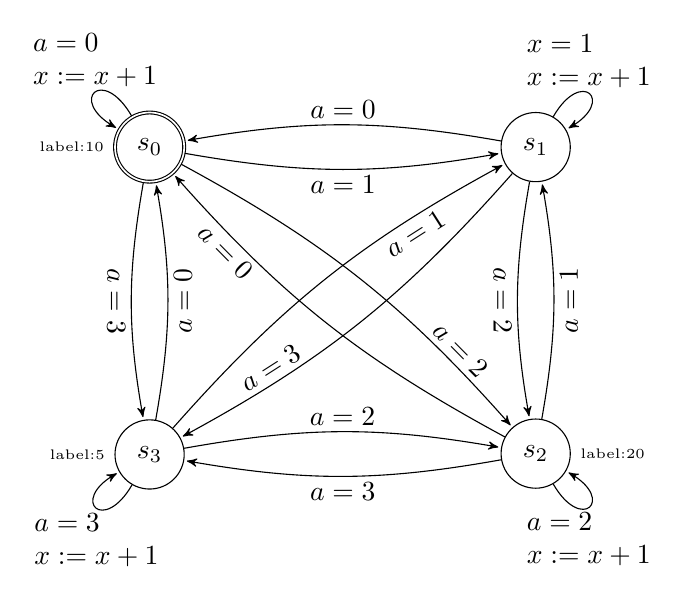
\begin{tikzpicture}[>=stealth',
    shorten > = 1pt,
node distance = 3cm and 4cm,
    el/.style = {inner sep=2pt, align=left, sloped},
every label/.append style = {font=\tiny}
                    ]
\node (q0) [state,accepting,label=left:{label:10}]  {$s_0$};
\node (q1) [state,right=of q0]                      {$s_1$};
\node (q2) [state,below=of q1,
            label=right:{label:20}]                 {$s_2$};
\node (q3) [state,below=of q0,
            label=left:{label:5}]                   {$s_3$};
\path[->] 
    (q0)  edge [in=150,out=120,loop] 
                node[el,above,rotate=-45] {$a=0$ \\ $x:=x+1$}   (q0)
    (q0)  edge [bend right=10]  node[el,below]  {$a=1$}         (q1)
    (q1)  edge [bend right=10]  node[el,above]  {$a=0$}         (q0)
    (q1)  edge [bend right=10]  node[el,below]  {$a=2$}         (q2)
    (q2)  edge [bend left=-10]  node[el,below]  {$a=1$}         (q1)
    (q0)  edge [bend right=10]  node[el,below]  {$a=3$}         (q3) 
    (q3)  edge [bend left=-10]  node[el,below]  {$a=0$}         (q0)
    (q0)  edge [bend left= 10]  node[el,above,pos=0.8] {$a=2$}  (q2)
    (q2)  edge [bend left= 10]  node[el,below,pos=0.8] {$a=0$}  (q0)
    (q1)  edge [bend left= 10]  node[el,above,pos=0.75] {$a=3$} (q3)
    (q2)  edge [bend left= 10]  node[el,below]  {$a=3$}         (q3)
    (q1)  edge [in=30, out=60,loop]  
                node[el,above,rotate=45] {$x=1$\\ $x:=x+1$}     (q1)
    (q3)  edge [bend left=10]   node[el,below,pos=0.75] {$a=1$} (q1)
    (q3)  edge [bend right=-10] node[el,above]  {$a=2$}         (q2)
    (q2)  edge [in=-30,out=-60, loop] 
                node[el,below,rotate=-45] {$a=2$ \\ $x:=x+1$}   (q2)
    (q3)  edge [in=-150,out=-120, loop] 
                node[el,below,rotate=45] {$a=3$ \\ $x:=x+1$}    (q3);
\end{tikzpicture}
\end{document}